\chapter{Analýza požadavků}

\textit{Tato kapitola popisuje požadavky, jež byly kladeny na vývoj systému.}

Cílem práce je vyrobit webovou aplikaci, která vizualizuje grafová data dle předem definovaných konfigurací a je schopna s těmito daty pracovat. Konfigurace popisují, jak a která data mají být vizualizována a jak je možné graf dále rozšiřovat. Celá aplikace bude rozdělena na klientskou a serverovou část, přičemž server odstiňuje klienta od RDF modelu a vrací mu již zpracovaná data.

Součástí požadavků na webovou aplikaci bylo vedoucím této práce připraveno několik konfigurací a webový server s určeným rozhraním, se kterým má klientská aplikace komunikovat.

V následujících kapitolách je nejprve popsána struktura konfigurací, rozhraní serveru a následně uživatelské požadavky na klientskou část aplikace.

\section{Konfigurace}

\textbf{Konfigurace} popisuje určitý pohled na data a definuje, jaká data lze v rámci této konfigurace vizualizovat a jakými způsoby. Konfigurace má \textbf{množiny pohledů}, kdy každá množina je aplikovatelná jen na určitou skupinu typů vrcholů podporovaných konfigurací. Množina pohledů pak obsahuje jednotlivé \textbf{pohledy}, které popisují, jak se na konkrétní vrchol můžeme dívat. Každý pohled pak určuje \textbf{náhled} (preview), \textbf{detail} a \textbf{expanzi}. Náhled poskytuje základní informace o vrcholu v rámci pohledu a určuje, jak má být vrchol v grafu vykreslen. Detail pak tyto informace rozšiřuje o další, které mohou být vypsány v tabulce. Expanze popisuje RDF graf, který doplňuje konkrétní vrchol o nové vztahy v rámci pohledu.

Konfigurace také určuje \textbf{počáteční vrchol} a \textbf{stylesheet}, tedy pravidla, jak mají být vrcholy v aplikaci vizualizovány.

Nakonec, konfigurace mohou být uloženy v rámci \textbf{meta konfigurací}, které slouží jako složky pro konfigurace.

Obrázek \ref{fig:configuration-class-diagram} popisuje UML diagram konfigurací.

\bigskip

Konfigurace jsou zapsány právě v RDF a slovník, jež je použit pro popis konfigurací, je popsán v následujícím textu.

\begin{figure}
    \centering
    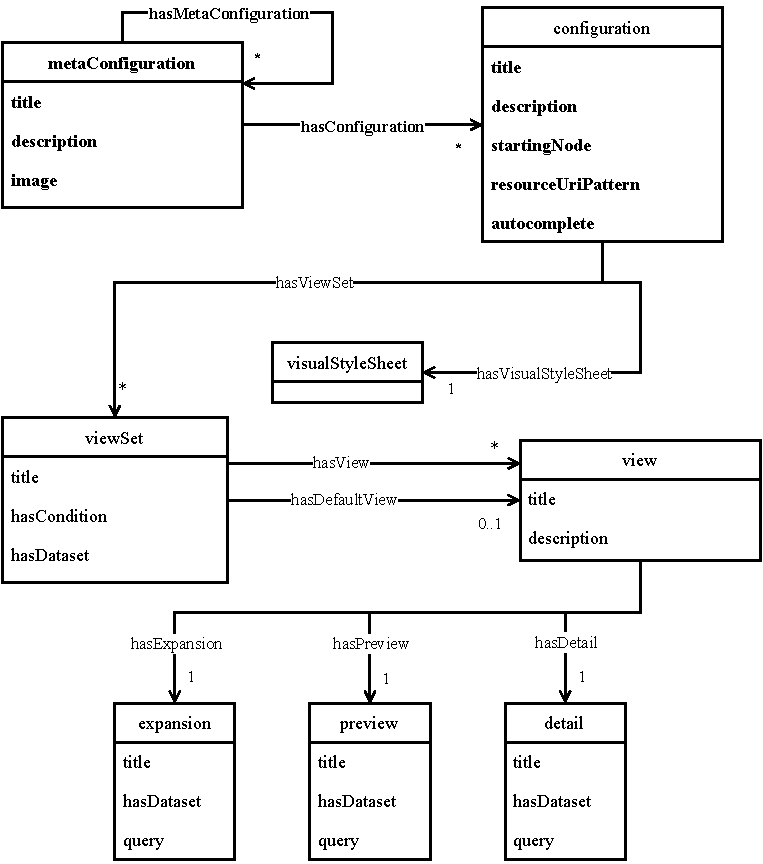
\includegraphics{media/configuration-class-diagram.pdf}
    \caption{Class diagram konfigurací včetně pozdější implementace meta konfigurace a rozšíření konfigurace.}
    \label{fig:configuration-class-diagram}
\end{figure}

\bigskip

V následujících sekcích jsou použity tyto RDF namespacy:
\begin{table}[h] \centering
\begin{tabular}{lp{10cm}}
\toprule
\multicolumn{1}{c}{Prefix} & \multicolumn{1}{c}{IRI}                                      \\
\midrule
browser                    & \texttt{\url{https://linked.opendata.cz/ontology/knowledge-graph-browser/}} \\
dct                        & \texttt{\url{http://purl.org/dc/terms/}}
\end{tabular}
\end{table}

\newpage

\subsection{Meta konfigurace} \label{pozadavky-metakonfigurace}
Meta konfigurace je skupina pro další konfigurace a meta konfigurace. Díky tomuto může uživatel procházet desítky různých konfigurací uspořádaných do složek obdobně jako v souborovém systému na počítači. Meta konfigurace má tyto vlastnosti:

\begin{itemize}
    \item \texttt{dct:title} Název meta konfigurace. \textit{(je možné zadat ve více jazycích)}
    \item \texttt{dct:description} Detailnější popis, co daná meta konfigurace zahrnuje. \textit{(je možné zadat ve více jazycích)}
    \item \texttt{browser:image} URL adresa s obrázkem reprezentující meta konfiguraci. Obrázek je pak zobrazen v aplikaci při procházení konfigurací.
    \item \texttt{browser:hasMetaConficuration} Meta konfigurace, které spadají pod tuto meta konfiguraci. \textit{(je očekáváno více objektů)}
    \item \texttt{browser:hasConfiguration} Konfigurace, které spadají pod tuto meta konfiguraci. \textit{(je očekáváno více objektů; popsáno dále)}
\end{itemize}

Meta konfigurací může být například \uv{Wikidata} nebo \uv{Otevřená data ČR}.

\subsection{Konfigurace} \label{pozadavky-konfigurace}
Konfigurace popisuje způsoby, jakými se lze dívat na data. Dvě konfigurace již byly zmíněny v úvodní kapitole. Jednalo se o procházení taxonů a slavných osobností na Wikidatech. Aktuálně může mít konfigurace tyto vlastnosti:

\begin{itemize}
    \item \texttt{dct:title} Název konfigurace. \textit{(je možné zadat ve více jazycích)}
    \item \texttt{dct:description} Detailnější popis čeho je možné s konfigurací dosáhnout. \textit{(je možné zadat ve více jazycích)}
    \item \texttt{browser:hasVisualStyleSheet} Určuje, jak mají být vrcholy v aplikaci vizualizovány. \textit{(popsáno dále)}
    \item \texttt{browser:startingNode} Doporučený vrchol nebo vrcholy, se kterými začít s procházením grafu. \textit{(je očekáváno více objektů)}
    \item \texttt{browser:resourceUriPattern} Regulární výraz popisující, jak by mělo vypadat IRI vrcholu. Používá se v aplikaci jako nápověda uživateli, zda zadal správné IRI dřív, než se pošle požadavek. Také se používá pro sestavení IRI z vyhledávaného dotazu, pokud lze dotazem nahradit část výrazu a získat tak validní IRI.
    \item \texttt{browser:hasViewSet} Seznam množin pohledů, které tato konfigurace podporuje. \textit{(popsáno dále)}
    \item \texttt{browser:autocomplete} JSON soubor se seznamem RDF vrcholů, podle kterých probíhá hledání. \textit{(je očekáváno více objektů; popsáno dále)}
\end{itemize}

\subsection{ViewSet} \label{pozadavky-view-sets}
View set reprezentuje skupinu pohledů. Skupina pohledů je vždy aplikovatelná na určité typy vrcholů v rámci konfigurace. View set má následující vlastnosti:
\begin{itemize}
    \item \texttt{dct:title} Název view setu. \textit{(je možné zadat ve více jazycích)}
    \item \texttt{browser:hasView} Pohledy, které patří pod tento view set. \textit{(je očekáváno více objektů; popsáno dále)}
    \item \texttt{browser:hasDefaultView} Výchozí pohled ze seznamu výše.
    \item \texttt{browser:hasCondition} SPARQL ASK dotaz, jež určí, zda tato množina pohledů je aplikovatelná na konkrétní vrchol.
    \item \texttt{browser:hasDataset} Dataset, vůči kterému probíhá ASK dotaz. \textit{(popsáno dále)}
\end{itemize}

\subsection{View} \label{pozadavky-view}
Konkrétní pohled na vrchol, který určuje náhled, detail a expanzi. Jak již bylo zmíněno v úvodu, pohledem může být například \uv{člověk, jež je autorem literárních děl}, nebo \uv{člověk jako součást rodokmenu}. View má následující vlastnosti:

\begin{itemize}
    \item \texttt{dct:title} Název pohledu. \textit{(je možné zadat ve více jazycích)}
    \item \texttt{dct:description} Popis pohledu. \textit{(je možné zadat ve více jazycích)}
    \item \texttt{browser:hasExpansion} Expanze -  popisuje graf který rozšiřuje vrchol o nové vrcholy v rámci daného pohledu. \textit{(popsáno dále)}
    \item \texttt{browser:hasPreview} Preview (náhled) - určuje data, která popisují vrchol v rámci daného pohledu a na základě kterých se vrchol vizuálně vykreslí. \textit{(popsáno dále)}
    \item \texttt{browser:hasDetail} Detail - určuje dodatečné informace o vrcholu v rámci daného pohledu. \textit{(popsáno dále)}
\end{itemize}

\subsection{Expanze} \label{pozadavky-expansion}
Expanze popisuje, jak lze daný vrchol rozšířit o nové vrcholy, které s ním souvisí. Expanze vrací graf. Expandované vrcholy tedy nemusí být přímými sousedy expandovaného vrcholu. Jako expanzi si můžeme představit například \uv{Zobraz všechny knihy, co napsala daná osoba}. Expanze formálně patří k pohledu (view).
\begin{itemize}
    \item \texttt{dct:title} Název expanze. \textit{(je možné zadat ve více jazycích, aktuálně se nepoužívá)}
    \item \texttt{browser:hasDataset} Popisuje dataset, vůči kterému se dotazuje na data. \textit{(popsáno dále)}
    \item \texttt{browser:query} Popisuje SPARQL CONSTRUCT dotaz, který bude spuštěn na endpointu datasetu a vrátí výsledný graf.
\end{itemize}

\subsection{Preview (náhled)} \label{pozadavky-preview}
Preview určuje, která data v rámci daného pohledu (view) popisují konkrétní vrchol. Popisem se myslí taková data, podle kterých se určí, jak bude vrchol na grafu vizuálně vykreslen. Obdobně jako expanze, preview patří ke konkrétnímu pohledu.

Preview má stejné vlastnosti jako expanze. \texttt{browser:query} v tomto případě popisuje SPARQL CONSTRUCT dotaz, který vrátí graf obsahující daný vrchol společně s literály ze kterých bude preview sestaven.

Konkrétně pro preview je predikát \texttt{browser:class} považován za třídu vrcholu. Podle těchto tříd je pak možné nastavovat vizuální styly pro konkrétní vrcholy a vrcholy s pomocí nich filtrovat.

\subsection{Detail} \label{pozadavky-detail}
Detail poskytuje dodatečné informace k vrcholu. Může se jednat o literály, které nemá smysl v dané konfiguraci vykreslit do grafu jako vrcholy, a proto budou zobrazeny v bočním panelu aplikace po kliknutí na vrchol.

Detail má stejné vlastnosti včetně \texttt{browser:query} jako preview.

\subsection{Dataset} \label{pozadavky-dataset}
Dataset popisuje SPARQL endpoint vůči kterému probíhá dotazování na data.

\begin{itemize}
    \item \texttt{dct:title} Název datasetu. \textit{(aktuálně se nepoužívá)}
    \item \texttt{void:sparqlEndpoint} URL adresa SPARQL endpointu na kterou se posílají dotazy.
    \item \texttt{browser:accept} Popisuje HTTP Accept type - v jakém formátu by měl endpoint svá data poskytnout.
\end{itemize}

\subsection{Visual style sheet} \label{pozadavky-visual-style-sheet}
Popisuje sadu pravidel, podle kterých budou vizuálně vykresleny vrcholy v aplikaci. Pravidla popsaná v rámci style sheetu mohou pracovat náhledem (preview) včetně zmíněných tříd. Forma zápisu stylů aktuálně odpovídá stylům, jaké používá knihovna Cytoscape\footnote{\url{https://js.cytoscape.org/}}, která bude popsána v další kapitole.

Visual style sheet má pouze jednu vlastnost

\begin{itemize}
    \item \texttt{browser:hasVisualStyle} Pravidlo popisující, jak se má provést stylování. Odkazuje na \textbf{Visual style}.
\end{itemize}

\subsubsection{Visual style}
Visual style má pak:

\begin{itemize}
    \item \texttt{browser:hasSelector} Selector pro Cytoscape knihovnu, jež vybírá, \\ na které vrcholy nebo hrany bude daný styl aplikován.
    \item \texttt{browser:*} Konkrétní styly, jak má být daný vrchol vykreslen. Používají se přesně ty názvy, které používá knihovna Cytoscape. Kupříkladu \\\texttt{browser:border-width} nebo \texttt{browser:background-color}.
\end{itemize}

\bigskip

Vedoucím projektu byly dodány pouze konfigurace. Výše sepsaná dokumentace konfigurací je již součástí této práce.

Původní návrh konfigurací byl mírně jednodušší a považoval konfigurace pouze jako odkazy na seznam pohledů. Klientská aplikace tedy musela mít seznam konfigurací s jejich názvy, počátečními vrcholy a dalšími parametry.

Na základě debaty s vedoucím byla konfigurace rozšířena o meta konfigurace a o parametry u konfigurace, jako název, popisek, počáteční vrcholy atp. To nám umožnilo mít v rámci klientské aplikace pouze jeden odkaz na IRI meta konfigurace, ze které se dají získat další meta konfigurace a konfigurace. Je tedy možné přidávat konfigurace bez nutnosti měnit klientskou část aplikace.

\bigskip

\begin{prikl}
Na závěr uveďme část konfigurace popisující procházení taxonů živočichů a rostlin na Wikidatech. Tato konfigurace je dostupná pod IRI \\\href{https://linked.opendata.cz/resource/knowledge-graph-browser/configuration/wikidata/animals}{https://linked.opendata.cz/resource/knowledge-graph-browser/}\\\href{https://linked.opendata.cz/resource/knowledge-graph-browser/configuration/wikidata/animals}{configuration/wikidata/animals}. Prefix \texttt{rb} definujme jako \\\url{https://linked.opendata.cz/resource/knowledge-graph-browser/}.

\smallskip

\textbf{Definice konfigurace}
\begin{code}
rb:configuration/wikidata/animals
    a browser:Configuration ;
    dct:title "Taxonomy of animals and plants"@en ,
              "Taxonomie rostlin a živočichů"@cs ;
    browser:hasVisualStyleSheet
        rb:wikidata/animals/style-sheet ;
    browser:startingNode <http://www.wikidata.org/entity/Q7377> ,
                         <http://www.wikidata.org/entity/Q192154> ;
    browser:resourceIriPattern
        "^http://www\\.wikidata\\.org/entity/Q[1-9][0-9]*$" ;
    browser:hasViewSet
        rb:view-set/wikidata/animals/taxon .
\end{code}
Jak již bylo popsáno v této kapitole, konfigurace má svůj název a popisek a definuje množiny pohledů, jak se na vrcholy dívat. V tomto případě se jedná pouze o jednu množinu. Mezi počátečními vrcholy jsou definovány dva a konfigurace nemá autocomlete, uživatel tedy může začít těmito dvěma vrcholy, nebo může ručně zadat IRI. Každá konfigurace má pak i stylesheet, který definuje barvy a tvary vrcholů při vykreslení na obrazovku.

\newpage

\textbf{Definice view setu}
\begin{code}
rb:view-set/wikidata/animals/taxon a browser:ViewSet ;
    dct:title "Views of taxons"@en ;
    browser:hasView rb:view/wikidata/animals/taxon/broader ,
                    rb:view/wikidata/animals/taxon/narrower ;
    browser:hasDefaultView rb:view/wikidata/animals/taxon/broader ;
    browser:hasCondition
        """PREFIX wd: <http://www.wikidata.org/entity/>
PREFIX wdt: <http://www.wikidata.org/prop/direct/>
ASK {
  ?node wdt:P31 ?type .
  FILTER(?type IN (wd:Q16521, wd:Q713623))
}""" ;
    browser:hasDataset rb:dataset/wikidata> .
\end{code}
Z ukázky si povšimněte \texttt{browser:hasCondition}, jež určuje, jaké vrcholy jsou na tuto množinu aplikovatelné. Přesně tento \texttt{ASK} dotaz byl popsán v příkladu v kapitole \ref{SPARQL}.

\medskip

\textbf{Definice pohledu}
\begin{code}
rb:view/wikidata/animals/taxon/narrower a browser:View ;
    dct:title "Child taxons"@en ;
    browser:hasExpansion rb:expansion-query/animals/taxon/narrower ;
    browser:hasPreview rb:preview-query/animals/taxon/basic ;
    browser:hasDetail rb:detail-query/animals/taxon/basic .
\end{code}

\textbf{Expanze} \\
Hodnota \texttt{browser:query} pro expanzi, jež je zmíněná v předchozím příkladu. Z dotazu byly vynechány prefixy.
\begin{code}
CONSTRUCT {
    ?childTaxon a wdab:taxon ;
                rdfs:label ?childTaxonLabel ;
                wdab:broader ?node ;
                browser:class "taxon",
                              ?childTaxonClass .

    wdab:broader browser:class "broader" .
} WHERE {
    ?childTaxon wdt:P171 ?node .

    OPTIONAL {
        ?childTaxon wdt:P105 ?childTaxonRank .
        ?childTaxonRank rdfs:label ?childTaxonRankLabel .
        FILTER(lang(?childTaxonRankLabel) = "en")
        BIND(IF(?childTaxonRank IN (wd:Q7432, wd:Q34740, wd:Q35409,
            wd:Q36602, wd:Q37517, wd:Q38348, wd:Q36732, wd:Q146481),
            ?childTaxonRankLabel, "unsupportedTaxon") AS
            ?childTaxonClass)
    }

    #FILTER(?childTaxonRank IN (wd:Q7432, wd:Q34740, wd:Q35409,
    wd:Q36602, wd:Q37517, wd:Q38348, wd:Q36732, wd:Q146481))
    SERVICE wikibase:label { bd:serviceParam wikibase:language "en". }
}
\end{code}
Povšimněte si, že expanze vrací přímo i preview všech expandovaných vrcholů, aby se omezila zátěž na datové zdroje.
\medskip

\textbf{Preview} \\
Hodnota \texttt{browser:query} pro preview, který je zmíněný v definici pohledu z předchozího příkladu. Z dotazu byly opět vynechány prefixy.
\begin{code}
CONSTRUCT {
    ?node a wdab:taxon ;
          rdfs:label ?nodeLabel ;
          browser:class "taxon",
                        ?taxonClass .
} WHERE {
    ?node wdt:P105 ?taxonRank .

    ?taxonRank rdfs:label ?taxonRankLabel .
    FILTER(lang(?taxonRankLabel) = "en")

    BIND(IF(?taxonRank IN (wd:Q7432, wd:Q34740, wd:Q35409, wd:Q36602,
        wd:Q37517, wd:Q38348, wd:Q36732, wd:Q146481), ?taxonRankLabel,
        "unsupportedTaxon") AS ?taxonClass)

    SERVICE wikibase:label { bd:serviceParam wikibase:language "en". }
}
\end{code}
Dotaz vypadá obdobně jako část předchozího dotazu, neboť expanze vrací pro každý vrchol i detail. Zde si můžeme povšimnout, jaké třídy dostává vrchol. Vždy se jedná o \uv{taxon}. Další třídy pak pocházejí z property, kterou Wikidata definují jako \uv{taxonomické zařazení} a jedná se například o \uv{species}, \uv{genus}, \uv{family} atp. Právě na \uv{genus} se aplikuje styl z ukázky dále a tedy všechny rody budou vykresleny žlutě.

\medskip

\textbf{Definice datasetu}
\begin{code}
rb:dataset/wikidata a void:Dataset ;
    dct:title "Wikidata SPARQL endpoint" ;
    void:sparqlEndpoint <https://query.wikidata.org/sparql> ;
    browser:accept "application/sparql-results+json" .
\end{code}

\textbf{Definice stylu}
\begin{code}
rb:wikidata/animals/style/genus a browser:VisualStyle ;
    browser:background-color "#ffbf00" ;
    browser:hasSelector ".genus" .
\end{code}

\newpage

\textbf{Detail} \\
Na závěr uveďme ještě detail, na který odkazuje pohled popsaný výše. Stejně jako expanze a náhled, i detail obsahuje titulek a odkaz na dataset, které opět pro přehlednost vynecháme a ukážeme pouze hodnotu \texttt{browser:query}, tedy dotaz na stažení detailu.
\begin{code}
CONSTRUCT {
    ?node rdfs:label ?nodeLabel ;
          wdt:P225 ?p225 ;
          wdt:P181 ?p181 ;
          wdt:P18 ?p18 .
} WHERE {
    node wdt:P31 wd:Q16521 .

    {
        ?node wdt:P225 ?p225 .
    } UNION {
        ?node wdt:P181 ?p181 .
    } UNION {
        ?node wdt:P18 ?p18 .
    }

    SERVICE wikibase:label { bd:serviceParam wikibase:language "en". }
}
\end{code}

Z ukázky vidíme, že mezi detail vrcholu patří popisek, název taxonu (\texttt{P225}), mapa rozšíření taxonu jako obrázek (\texttt{P181}) a obecný obrázek (\texttt{P18}). Klientská aplikace pak může tyto dva obrázky stáhnout a vykreslit je v bočním panelu při kliknutí na vrchol.
\end{prikl}

\newpage

\section{Server}
Dalším požadavkem bylo, aby klientská aplikace komunikovala se serverem, který provádí dotazy a vrací data pro aplikaci. Server bude detailněji popsán v příští kapitole.

Server zprostředkovává následující požadavky:
\begin{itemize}
    \item \texttt{/meta-configuration} - Vrátí informace o meta konfiguraci.

    \item \texttt{/configuration} - Vrátí informace o konfiguraci.

    \item \texttt{/stylesheet} - Vrátí visual style sheet.

    \item \texttt{/view-sets} - K vrcholu a konfiguraci vrátí seznam view setů.

    \item \texttt{/preview} - K vrcholu a pohledu vrátí preview.

    \item \texttt{/detail} - K vrcholu a pohledu vrátí detail.

    \item \texttt{/expand} - K vrcholu a pohledu vrátí expandované vrcholy.
\end{itemize}

\newpage







\begin{figure}
    \centering
    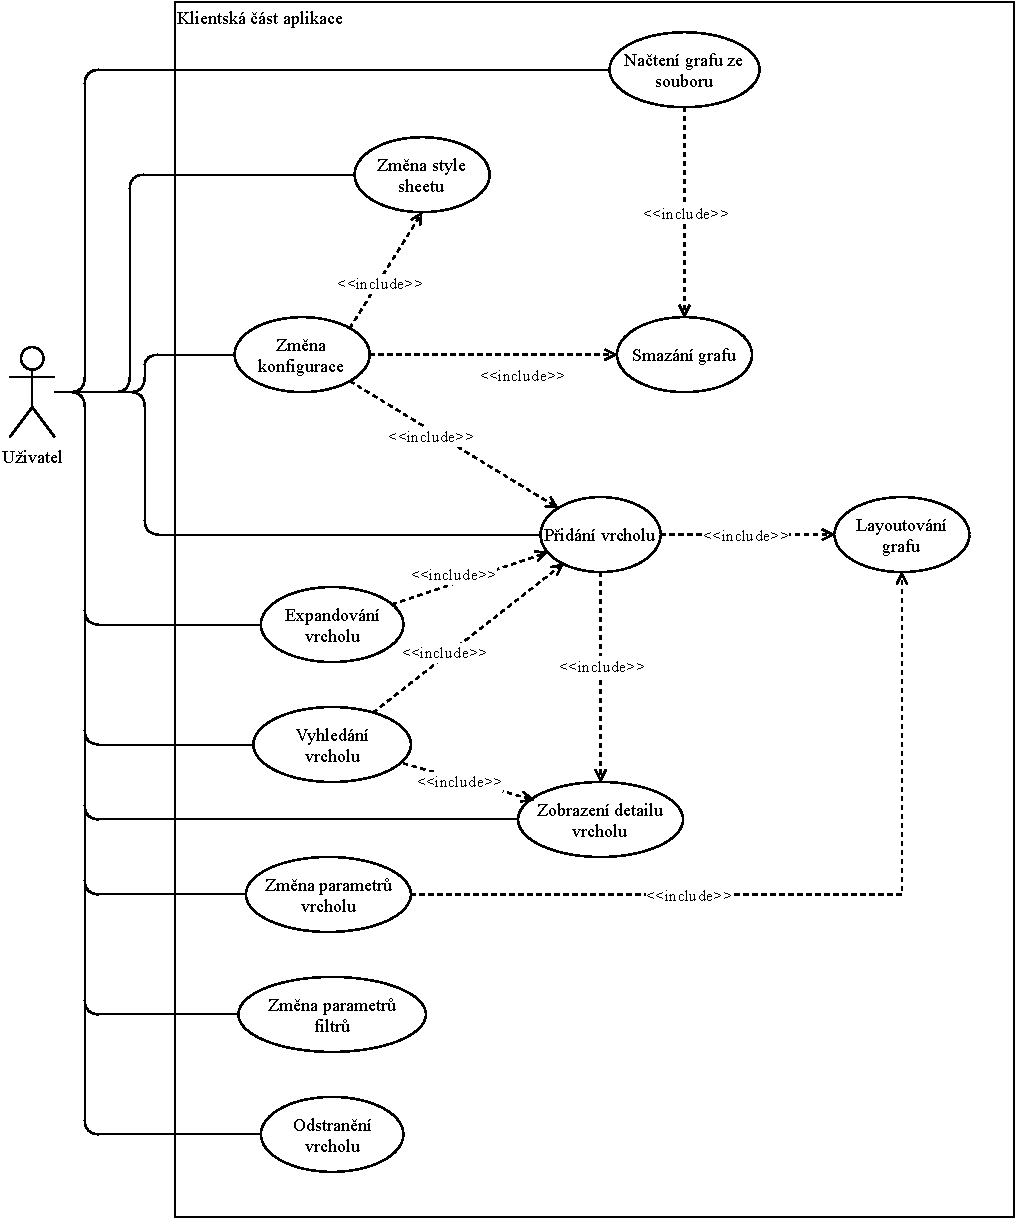
\includegraphics[width=\textwidth]{media/use-case.pdf}
    \caption{Use case diagram dle uživatelských požadavků.}
    \label{fig:use-case}
\end{figure}

\section{Uživatelské a systémové požadavky}\label{pozadavky-uzivatelske}

Níže je sepsán seznam původních požadavků na klientskou aplikaci.

\subsection*{Konfigurace a stylesheet}
Uživatel musí být schopen vybrat IRI konfigurace a IRI visual style sheetu a lze je kdykoli změnit. IRI konfigurace může být vybráno jen jedno.

\paragraph{Analýza} Konfigurace popisuje, jak je graf zobrazen a které pohledy jsou na vrcholy aplikovatelné. Ačkoli by teoreticky bylo možné podporovat dvě konfigurace, nebudeme toto implementovat. Změna konfigurace tedy smaže aktuální graf a vytvoří graf nový.

\subsection*{Vložení vrcholů}
Uživatel může ručně zadat IRI vrcholu, který se následně zobrazí v grafu.

\paragraph{Analýza} Pro úspěšné zobrazení vrcholu musí aplikace znát jeho \texttt{preview}. To lze ale získat pouze z konkrétního pohledu a je tedy nutné nejprve stáhnout \texttt{view-sets} daného vrcholu, z nich následně vybrat defaultní a zvolit výchozí pohled. Pak je možné zavolat metodu \texttt{preview} na serveru a získat data o vrcholu.

\begin{itemize}
    \item IRI vrcholu bude považováno za chybné, pokud server vrátí prázdnou množinu na dotaz \texttt{view-sets}. V takovém případě totiž nejde aplikovat žádné pohledy na vrchol, a tedy zřejmě nepatří do dané konfigurace.
    \item Vrchol může být již v grafu přítomen, pak se označí a přesune se na něj obrazovka. Pokud je vrchol skrytý, bude odkryt. Pokud jsou zapnuté filtry a vrchol je skrytý filtrem, vrchol se v grafu nezobrazí. Pokud se vrchol podaří načíst, nebo již existuje, bude vybrán a zobrazí se jeho detail v pravém panelu.
\end{itemize}

\subsection*{Detail vrcholu}
Pokud uživatel klikne na vrchol, zobrazí se panel s podrobnými informacemi o vrcholu. Bude zobrazen detail vrcholu voláním metody \texttt{detail} na serveru a budou zobrazeny veškeré pohledy vrcholu, možnost je přepínat a provádět expanze podle daného pohledu.

Detail bude zobrazen jako dvousloupcová tabulka klíč-hodnota.

Panel bude zobrazovat také další možné akce k vrcholu.

\paragraph{Analýza} Vrchol nemusí mít načtené \texttt{view-sets}, \texttt{preview} ani \texttt{detail}, je tedy nutné po zobrazení panelu tyto informace stáhnout a během stahování zobrazit informaci, že se data stahují.

Může se stát, že \texttt{view-sets} vrátí prázdný výsledek. V takovém případě vrchol v grafu necháme i přes to, že podle původního požadavku bychom jej smazali. Taková situace nicméně implikuje chybně napsanou konfiguraci a uživatel bude o tomto informován chybovou hláškou.

Mezi akcemi bude lokalizace vrcholu, smazání, opětovné načtení všech dat, zafixování pozice.

\subsection*{Skrývání vrcholů}
Uživatel může skrývat vrcholy v panelu s detailem. Skrytý vrchol se v grafu skryje společně se všemi hranami. Bude možné zobrazit seznam skrytých vrcholů ze kterého půjde skryté vrcholy opět zviditelnit.

\paragraph{Analýza} Bude přidáno tlačítko k detailu pro skrytí/zobrazení vrcholu. Současně pro vetší přehlednost bude do detailu přidána hláška informující uživatele, že je vrchol skrytý.

Skryté vrcholy nebude možno lokalizovat, ale stále bude možné s nimi dále pracovat. Podle prvního požadavku se vrchol opět zobrazí, pokud ho uživatel bude chtít explicitně vložit.

V panelu se skrytými vrcholy bude možnost vrcholy přímo zobrazit, nebo si zobrazit jejich detail. Detail skrytého vrcholu funguje stejně jako pro viditelné vrcholy.

\subsection*{Expanze}
Po dvojkliku na vrchol se vrchol expanduje podle aktuálního pohledu. vrchol je také možné expandovat v panelu s detailem kliknutím na tlačítko expanze u příslušného pohledu. Expanzí se zavolá metoda \texttt{expand} na serveru a v grafu se zobrazí nové vrcholy.

\paragraph{Analýza} Pokud přidávaný vrchol v grafu již je a je skrytý, pak skrytým zůstane. Na rozdíl od přidávání jednoho vrcholu totiž explicitně neříkáme, že chceme daný vrchol přidat. Protože je možné vrcholy mazat, povolíme uživateli provádět expanzi znova, i když již byla provedena.

Budeme si také pamatovat které vrcholy a hrany vznikly ze které expanze pro snazší práci s expanzemi.

\subsection*{Filtrování vrcholů}
Uživatel může přidat filtr, jež skryje nevyhovující vrcholy. Takovéto skryté vrcholy se pak chovají stejně jako uživatelem skryté vrcholy. Požadované filtry jsou
\begin{itemize}
    \item Zobraz jen ty vrcholy, jež mají stupeň v daném intervalu nebo rozmezí.
    \item Zobraz vrcholy jen s konkrétním typem nebo třídou.
\end{itemize}

\paragraph{Analýza} Aplikace by měla podporovat snadné přidání filtrů do budoucna a podporu pro pluginy, které dodávají vlastní možnosti filtrování. Aby bylo možné vyjádřit libovolné filtry, každý filtr by měl mít přístup k celému grafu a všem vrcholům.

Vrchol může být skrytý jak filtrem, tak i uživatelem. Pro přehlednost by měl být uživatel informován, že nemůže ručně zobrazit vrchol který je skrytý filtrem. Tyto vrcholy budou stále zobrazeny v seznamu skrytých vrcholů pro možnost přístupu k nim.

Každý filtr určí, zda je vrchol podle tohoto filtru viditelný. Vrchol pak bude viditelný, pokud všechny filtry určí, že viditelný je. Jedná se tedy o konjunkci.

Typy a třídy vrcholů nejsou známy předem a API serveru neumožňuje získat celou množinu typů a tříd. Je tedy nutné přizpůsobit filtry tak, aby si dokázaly poradit s novými vrcholy. Proto filtry na typ a třídu budou mít dva módy. V jednom módu explicitně skrývají zvolené vlastnosti a ve druhém explicitně zobrazují vrcholy s danými vlastnostmi. Toto chování pak ovlivní přidání nových, neznámých, vrcholů. V prvním případě nový vrchol bude zobrazen (pokud jeho typ, resp. třídy ještě nejsou známy) a ve druhém případě bude ihned skryt.

\subsection*{Vícejazyčné uživatelské rozhraní}
Uživatel může přepínat mezi více jazyky uživatelského rozhraní. Aktuálně bude podporována pouze angličtina a čeština.

\paragraph{Analýza} Kromě uživatelského rozhraní by měl být vícejazyčný i graf. Aktuální API serveru toto ještě neumožňuje a problém je předmětem poslední kapitoly. Multijazyčnost zatím podporují metody \texttt{meta-configuration} a \texttt{configuration} na serveru. Protože obecně můžou existovat překlady do spousty světových jazyků, je vhodné stahovat pouze požadovaný jazyk a při jeho změně stáhnout data s novým jazykem znovu.

Pro velké grafy může být překlad problémem, protože změna jazyku může vyvolat spoustu požadavků na datové zdroje. Pro překlad grafu by tedy bylo nejlepší stáhnout překlad až když si uživatel zobrazí detail, nebo explicitně neoznačí vrcholy na překlad. Taktéž je vhodné oddělit výběr jazyka pro obsluhu aplikace a výběr konfigurací od překladu jednotlivých vrcholů. Příkladem situace, kde je oddělení žádoucí, může být procházení měst v Japonsku anglicky mluvícím uživatelem. V této situaci bychom požadovali, aby názvy měst byly v originálním jazyce.

Překlady do konkrétního jazyka by měly být v jednom souboru, nebo adresáři a přidávání nových jazyků by mělo být snadné, nejlépe bez zásahu do kódu aplikace.

\subsection*{Stažení grafu do souboru}
Uživatel má možnost stáhnout aktuální graf do souboru a později ho ze souboru načíst zpět.

\paragraph{Analýza} Protože je aplikace ve vývoji, je třeba dbát na zpětnou kompatibilitu. Při každé nové verzi je tedy třeba ověřit, zdali soubor pochází ze staré verze a použít staré metody pro jeho zpracování a převedení do nového systému. Výsledný soubor může být zkomprimován pro menší velikost a nabízí se i možnost stáhnout jen základní informace tak, aby zbytek mohl být při načtení stažen ze serveru.

Pokud uživatel bude chtít zavřít aplikaci, bude dotázán, zda chce aktuální graf uložit do souboru. Uložený graf již nebude blokovat stránku o uzavření, dokud uživatel nesmaže, nebo nepřidá nové vrcholy. Stažení detailu, nebo změna pohledu nebude považována za změnu hodnou k uložení.

Pokud uživatel zvolí načtení nového souboru, starý graf bude zahozen a uživatel tedy bude požádán o uložení.

Kromě otevření souboru ze systému bude možnost soubor načíst i z webu.

\subsection*{Odstranění vrcholu}
Uživatel může z grafu vrchol odstranit.

\paragraph{Analýza} Odstraněním vrcholu se musí odstranit i všechny hrany patřící vrcholu. Vrchol by také měl být odstraněn ze všech expanzí tak, aby nedocházelo k únikům paměti.

Odstranit vrchol bude možné pomocí tlačítka v panelu s detailem, popřípadě skupinu vrcholů bude možné odstranit obdobným způsobem.

\subsection*{Vyhledávání vrcholů s pomocí autocomplete}
Pokud to konfigurace umožňuje, bude možné přidávat nové vrcholy do grafu s pomocí autocomplete.

\paragraph{Analýza} Data pro vyhledávání se budou stahovat až když uživatel bude chtít poprvé vyhledávat.

Návrh vyhledávače by měl podporovat více vyhledávacích zdrojů a vhodně kombinovat nalezené výsledky v případě, že více zdrojů vrátí stejné vrcholy.

Kromě vyhledávání v JSON souboru se pak nabízí hledat i v aktuálním grafu a umožnit uživateli zadat do vyhledávacího pole přímo IRI vrcholu, popřípadě její část, ze které se aplikace pokusí sestavit celou IRI.
\bigskip

Níže jsou požadavky dodané do aplikace později.

\subsection*{Podpora layoutů}
Aplikace bude umožňovat několik způsobů layoutování grafu, které si bude moci uživatel volit.

\begin{itemize}
    \item Pokud to layout umožňuje, bude možné ukotvit vrchol. To lze provést přesunutím vrcholu, pravým kliknutím myši, nebo z nabídky u detailu vrcholu. U ukotvených vrcholů bude zobrazena ikonka. Takovéto vrcholy pak nebudou layoutem ovlivněny.
    \item Layout reaguje na různé události, jako vytvoření skupiny, expanze vrcholu, přidání nového vrcholu do grafu, přesunutí vrcholu a na základě těchto událostí provádí layoutování grafu.
    \item Pokud to layout umožňuje, bude v pravém dolním rohu obrazovky tlačítko, které spustí layoutování explicitně.
    \item Layout má vlastní nastavení.
\end{itemize}

\subsection*{Seskupování vrcholů}
Vrcholy bude možné seskupovat do skupin, které budou ve vizuálním grafu reprezentovány jedním vrcholem. Pokud expanze vrátí větší množství nových vrcholů, vzniknou jako skupina. Skupinu bude možné rozbít dvojklikem.

\begin{itemize}
    \item Z grafového hlediska skupina vznikne kontrakcí hran mezi vrcholy skupiny. To znamená, že pokud vedla hrana mezi vrcholem mimo skupinu a vrcholem ve skupině, povede tato hrana mezi vrcholem mimo skupinu a skupinou. Všechny násobné hrany stejného typu budou nahrazeny jednou hranou. Obdobně toto platí pro hrany mezi dvěma skupinami. Pokud je ve skupině vrchol skrytý (uživatelem, nebo filtrem), jeho hrany se nepodílejí na utváření skupiny. Pokud jsou všechny vrcholy skupiny skryty, je skrytá i skupina.
    \item Skupina se na grafu chová jako obyčejné vrcholy, je ji možné skrýt, přesouvat, ukotvit atp.
    \item Označením několika vrcholů se nabídne možnost vytvořit skupinu. Tato skupina pak vznikne na místě, kde byly původní vrcholy.
    \item Rozbít skupinu je možné dvojklikem, nebo tlačítkem z detailu skupiny. Vrchol skupiny bude odstraněn a vzniknou místo něj původní vrcholy, které budou layoutovány.
\end{itemize}

\subsection*{Kompaktní mód}
Uživatel bude mít možnost zapnout kompaktní mód. Během něj se ve středu obrazovky zobrazí pouze zvolené vrcholy a jejich přímí sousedi. Tyto vrcholy budou layoutovány bez ohledu na ostatní vrcholy, které budou skryté. Uživatel pak bude mít možnost graf v tomto módu procházet klikáním na sousedy aktivního vrcholu.

\paragraph{Analýza} Kompaktní mód se vypne, pokud nebude vybrán žádný vrchol. Při kompaktním módu se bude obrazovka neustále zaměřovat na vrcholy účastnící se kompaktního módu. Jakmile vrchol kompaktní mód opustí, měl by se vrátit na svou původní pozici. Po skončení kompaktního módu se původní rozložení grafu nezmění. Nově vytvořené vrcholy v rámci kompaktního módu musí být správně umístěny, jakmile bude mód ukončen.
